\section{Data Processing}
\label{sec:data-processing}

\subsection{Trigger}
As described in section \ref{sec:dom-daq}, the high-frequency ATWD waveform digitization in each DOM is triggered when it and its adjacent or next-to-adjacent neighbors on the same string record a voltages of at least 0.25 PE-equivalent within a $\pm$1~$\mu$s time window, which is referred to as the Hard Local Coincidence (HLC) condition. Data acquisition for DeepCore is triggered when this condition is fulfilled for at least three DOMs inside the DeepCore fiducial volume within a $\pm$2.5~$\mu$s window. If this condition is met, the waveforms for all DOMs that have observed voltages of at least 0.25~PE within a $\pm$10~$\mu$s time window centered around the trigger time are recorded. A DOM that is included in this readout but for which the HLC condition has not been met is said to fulfill the \emph{Soft Local Coincidence} (SLC) condition. The DeepCore trigger rate is less than 10~Hz and will trigger on \~70\% of $\nu_\mu$ events at 10~GeV and >90\% of $\nu_\mu$ events at 100~GeV\cite{DeepCore}.

\subsection{Online Filter}

Once the trigger condition is met, the recorded waveforms within the trigger window are converted into reconstructed pulses and are then passed into a set of \emph{online} filters (i.e. filters running on hardware at the Pole). These filters are each designed to select events that are relevant to different physics measurements that are performed within the IceCube collaboration. For the purposes of the analysis presented in this thesis, events are selected using the \emph{DeepCore filter}. This filter is designed to select events that start inside the DeepCore fiducial volume and to reject those that are consistent with muons entering the detector from the outside.
\begin{marginfigure}
    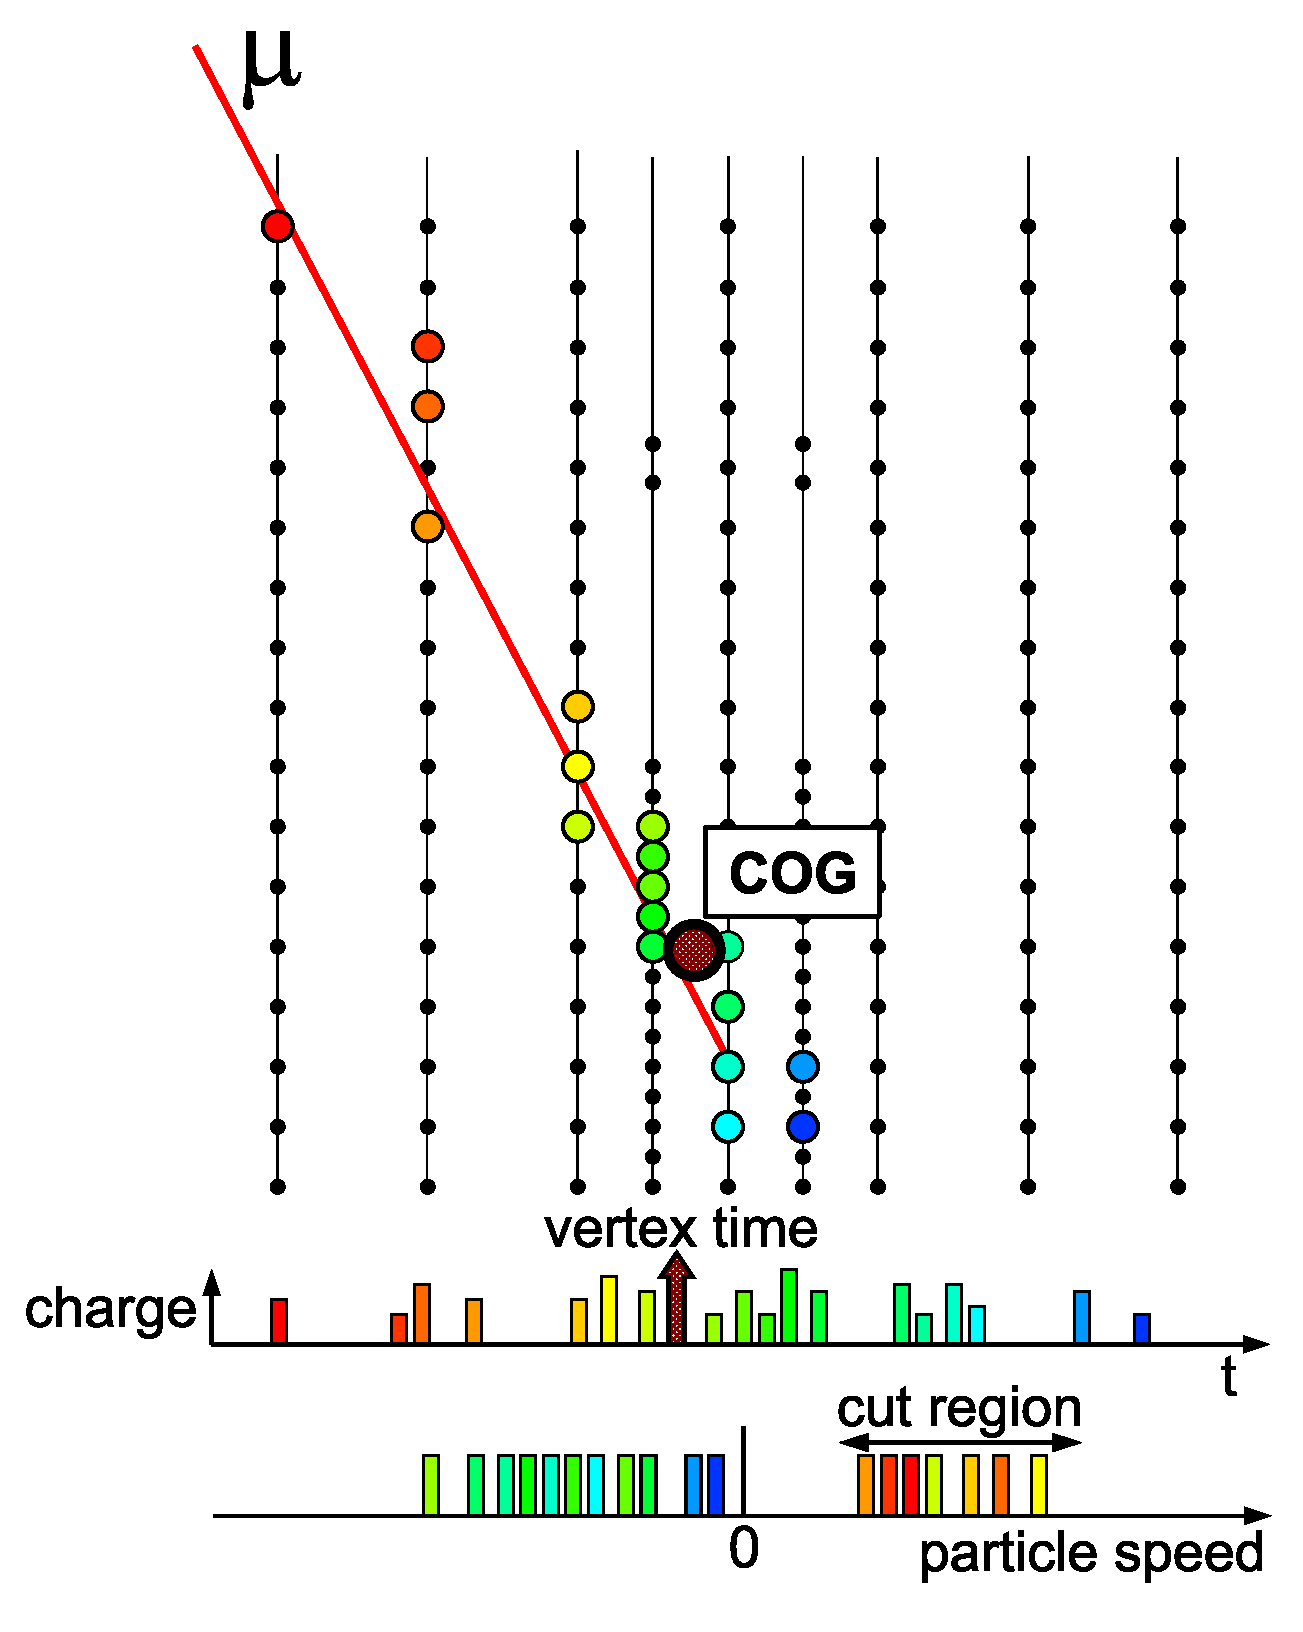
\includegraphics[width=\textwidth]{figures/icecube/eventviews/FilterDiagram.pdf}
    \caption{Example of an event that would be rejected by the online filter algorithm. DOMs that have observed light are highlighted in color depending on time from red (early hits) to blue (late hits). DOMs that have not observed any light are shown as black dots. Figure taken from \cite{DeepCore}.}
    \label{fig:online-filter-event}
\end{marginfigure}
The filter first applies a noise cleaning algorithm based on a coincidence condition between hits on different DOMs, where hits in DOMs for which the HLC condition was met are always kept. The cleaned hit series is split between those hits that fall within the DeepCore fiducial volume and those outside of it. The veto algorithm then calculates the COG in space and time of the hits inside the fiducial volume and then the velocity that a signal would have to travel from each hit occurring outside the fiducial volume to coincide with the COG. If this velocity is close to the speed of light (between $0.25\;\mathrm{ns/s}$ and $0.4\;\mathrm{ns/s}$) for at least one hit, the event is rejected because it is consistent with a muon traveling through the veto region and entering DeepCore. Figure~\ref{fig:online-filter-event} shows an example of an event that would be rejected by the online filter. Only events passing the trigger and filter condition are sent North via satellite for further \emph{offline} filtering.

\subsection{Offline Filter}

The offline filter is separated into subsequently applied \emph{levels}, referred to as L3, L4, and L5, where each level reduces the amount of background (atmospheric muons and noise) by approximately an order of magnitude while keeping most of the DeepCore starting events that are the target of the selection.

\subsubsection{Level 3}
At the lowest offline filter level, L3, cuts are applied to simple variables that remove the most easily identifiable background events while using only few computational resources. The variables aimed at cutting noise consist mostly of different DOM hit counts within hit series to which noise cleaning algorithms have been applied. The cuts aimed at removing muons consist of conditions on the number of hits in the veto region as well as conditions on the vertical position of the first HLC hit. The distribution for one of the variables used in the L3 filter is shown in figure~\ref{fig:l3-var-cleaned-full-time-length}. It is apparent from the distributions that there is a significant population of events in data with large values of the plotted variable that does not exist in simulation. These events are discarded, improving the agreement between data and simulation for events passing the L3 filter.
\begin{figure}
    \centering
    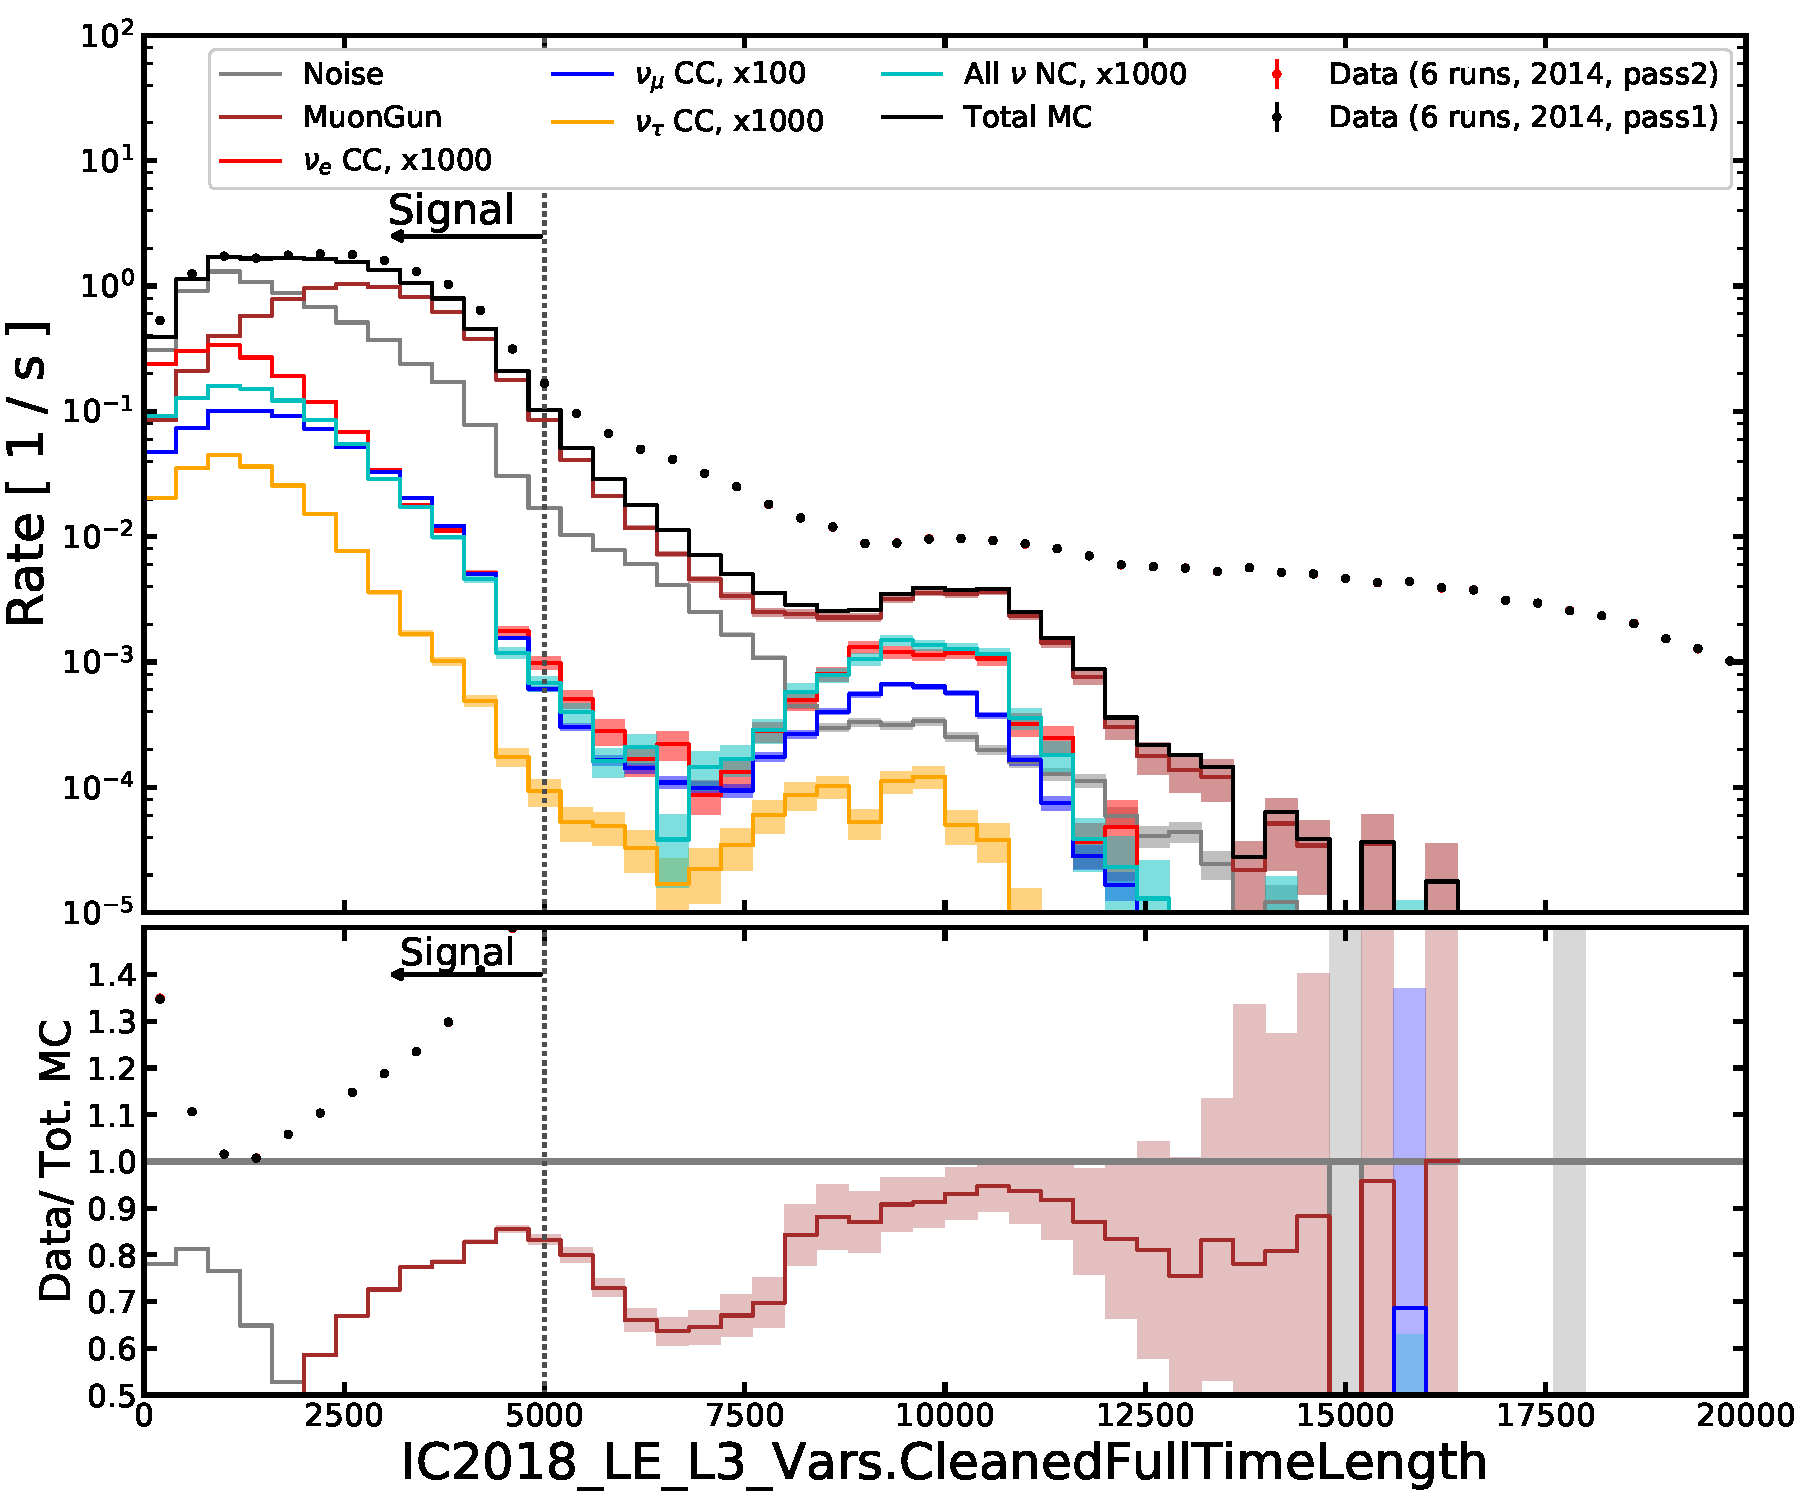
\includegraphics[width=7 cm]{figures/icecube/selection/IC2018_LE_L3_Vars_CleanedFullTimeLength.pdf}
    \caption{Distribution of one of the variables used in the L3 offline filter, the time between the last hit and the first hit after noise cleaning. Histograms show the distributions in simulated data separated by particle and interaction type, data points with error bars show the distribution of real data. The bottom panel shows the ratio between data and simulation. Events falling on the "signal" side of the histogram are passed to the next filter level.}
    \label{fig:l3-var-cleaned-full-time-length}
\end{figure}

\subsubsection{Level 4}
In the next level, L4, more advanced selections based on the output of Boosted Decision Trees (BDTs) are applied, with a separately trained BDT for noise and muon rejection, respectively. The output of each BDT is a probability score between zero (background-like) and one (signal-like).  The inputs into the BDT aimed at noise rejection consist of hit counts in cleaned hit series and variables that characterize the geometric and temporal spread of the observed hits, such as the full width half maximum (FWHM) of the hit times. The BDT is trained using simulated pure noise and neutrino events. Events are passing the L4 noise cut if the BDT score is above 0.7, which reduces the number of pure noise events by two orders of magnitude from 36.6~mHz to approximately 0.3~mHz. The BDT that is used to reject atmospheric muons also takes simple variables as its input that consist mostly of different veto hit counts and variables that characterize the distribution of z-coordinates of the observed hits as well as their radial distance with respect to the center of the DeepCore fiducial volume. In contrast to the noise BDT, however, the muon BDT is trained using real data and simulated neutrino events, with the goal of rejecting data events. This is possible because the data sample consists to 99\% of atmospheric muons at this stage of the event selection. Events are passing the L4 muon cut if the output score from the muon BDT is above 0.65, removing 94\% of all muon events while keeping 87\% of all neutrinos. The distributions of the output scores of both BDTs are shown in figure~\ref{fig:l4-bdt-output}.
\begin{figure*}
    \centering
    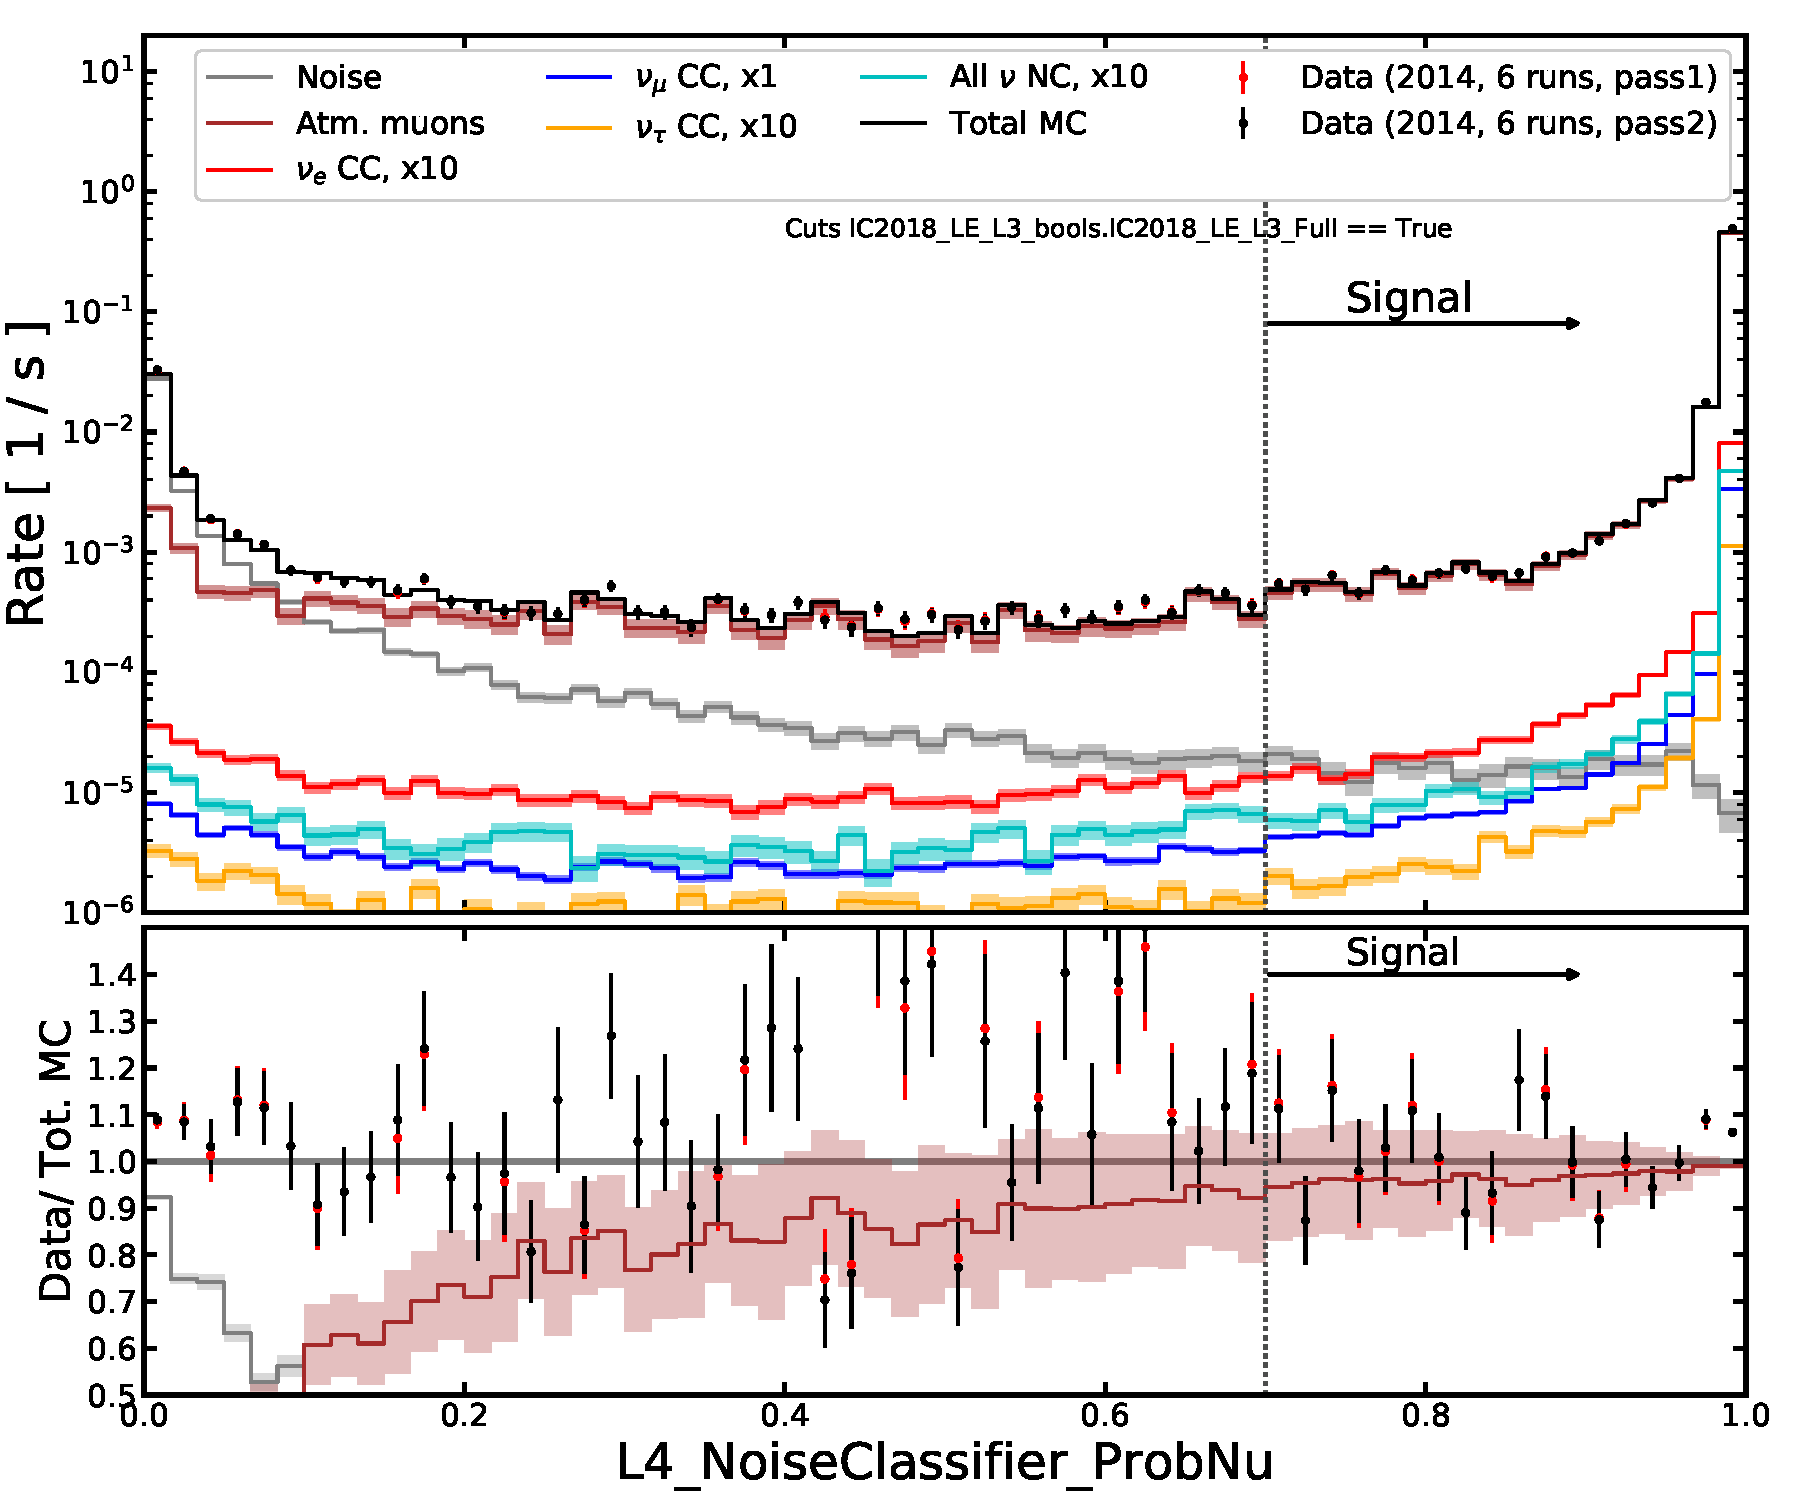
\includegraphics[width=7 cm]{figures/icecube/selection/L4_noiseBDT_L4_NoiseClassifier_ProbNu.pdf}
    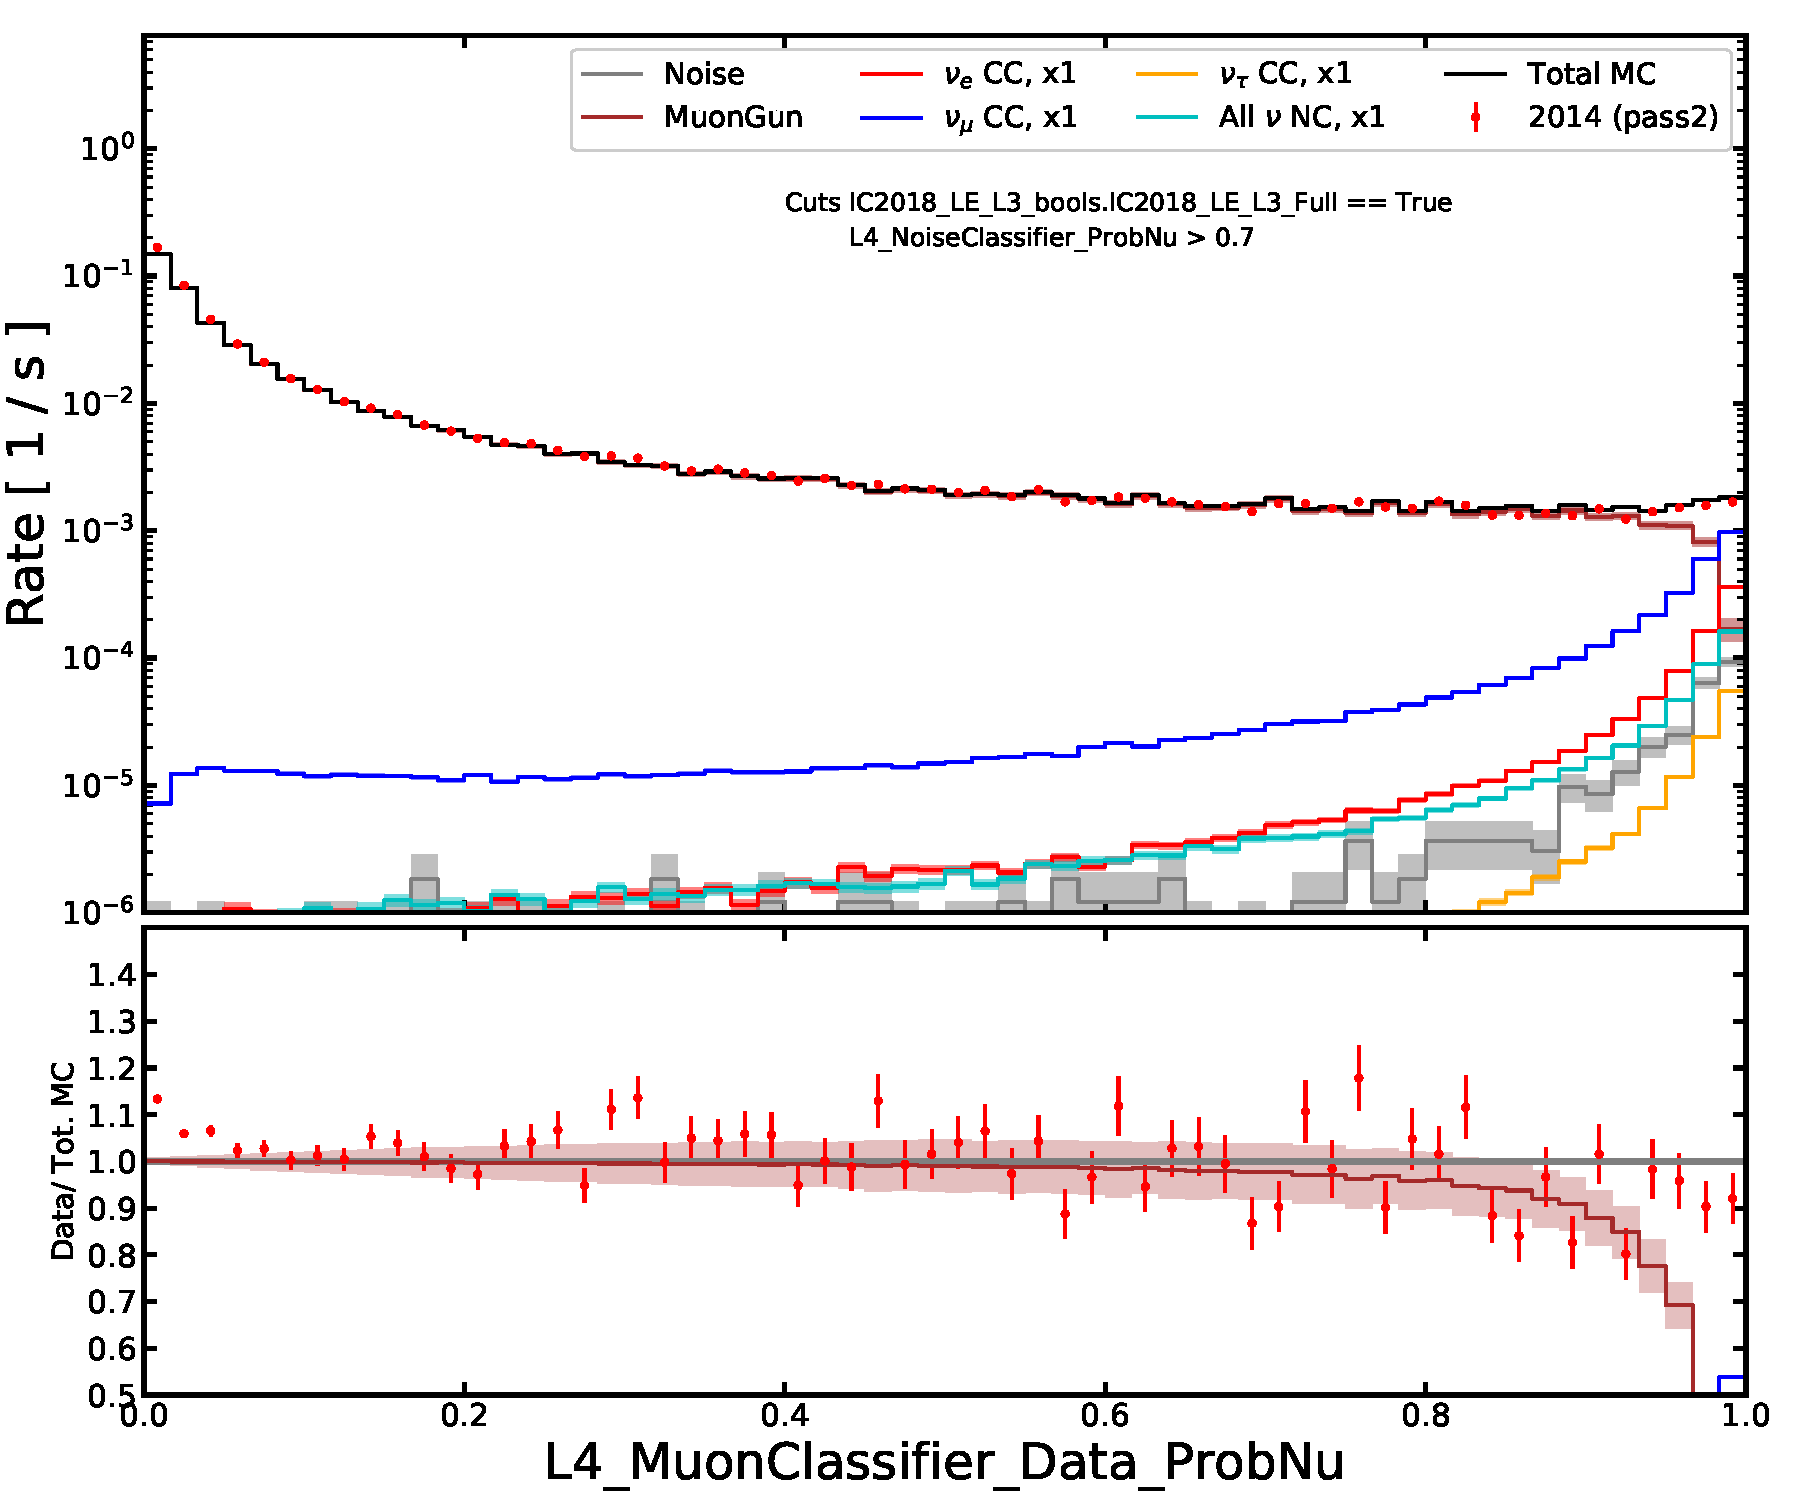
\includegraphics[width=7 cm]{figures/icecube/selection/L4_muon_L4_MuonClassifier_Data_ProbNu.pdf}
    \caption{Distribution scores for the noise (left) and muon (right) BDT. The distributions of the muon classifier are shown for events where the score of the noise BDT is greater than 0.7.}
    \label{fig:l4-bdt-output}
\end{figure*}

\subsubsection{Level 5}
The final offline filter level that is applied before the event reconstruction step is L5. This filter searches specifically for hits occurring in un-instrumented \emph{corridors} within the IceCube array through which an atmospheric muon can sneak into the DeepCore volume while evading previous veto cuts. In addition, events with more than seven hits in the outermost strings of the IceCube array or that have a down-going pattern of hits in the uppermost region of the detector are vetoed to remove events containing atmospheric muons entering the detector coincidentally with neutrinos. The distribution for one of the corridor variables and one of the muon rejection variables are shown in figure~\ref{fig:l5-vars}. Table~\ref{tab:l5_summary} shows the rates of each event type expected at each level of the selection up to L5 together with the efficiency of the filter at the final level.
\begin{figure*}
    \centering
    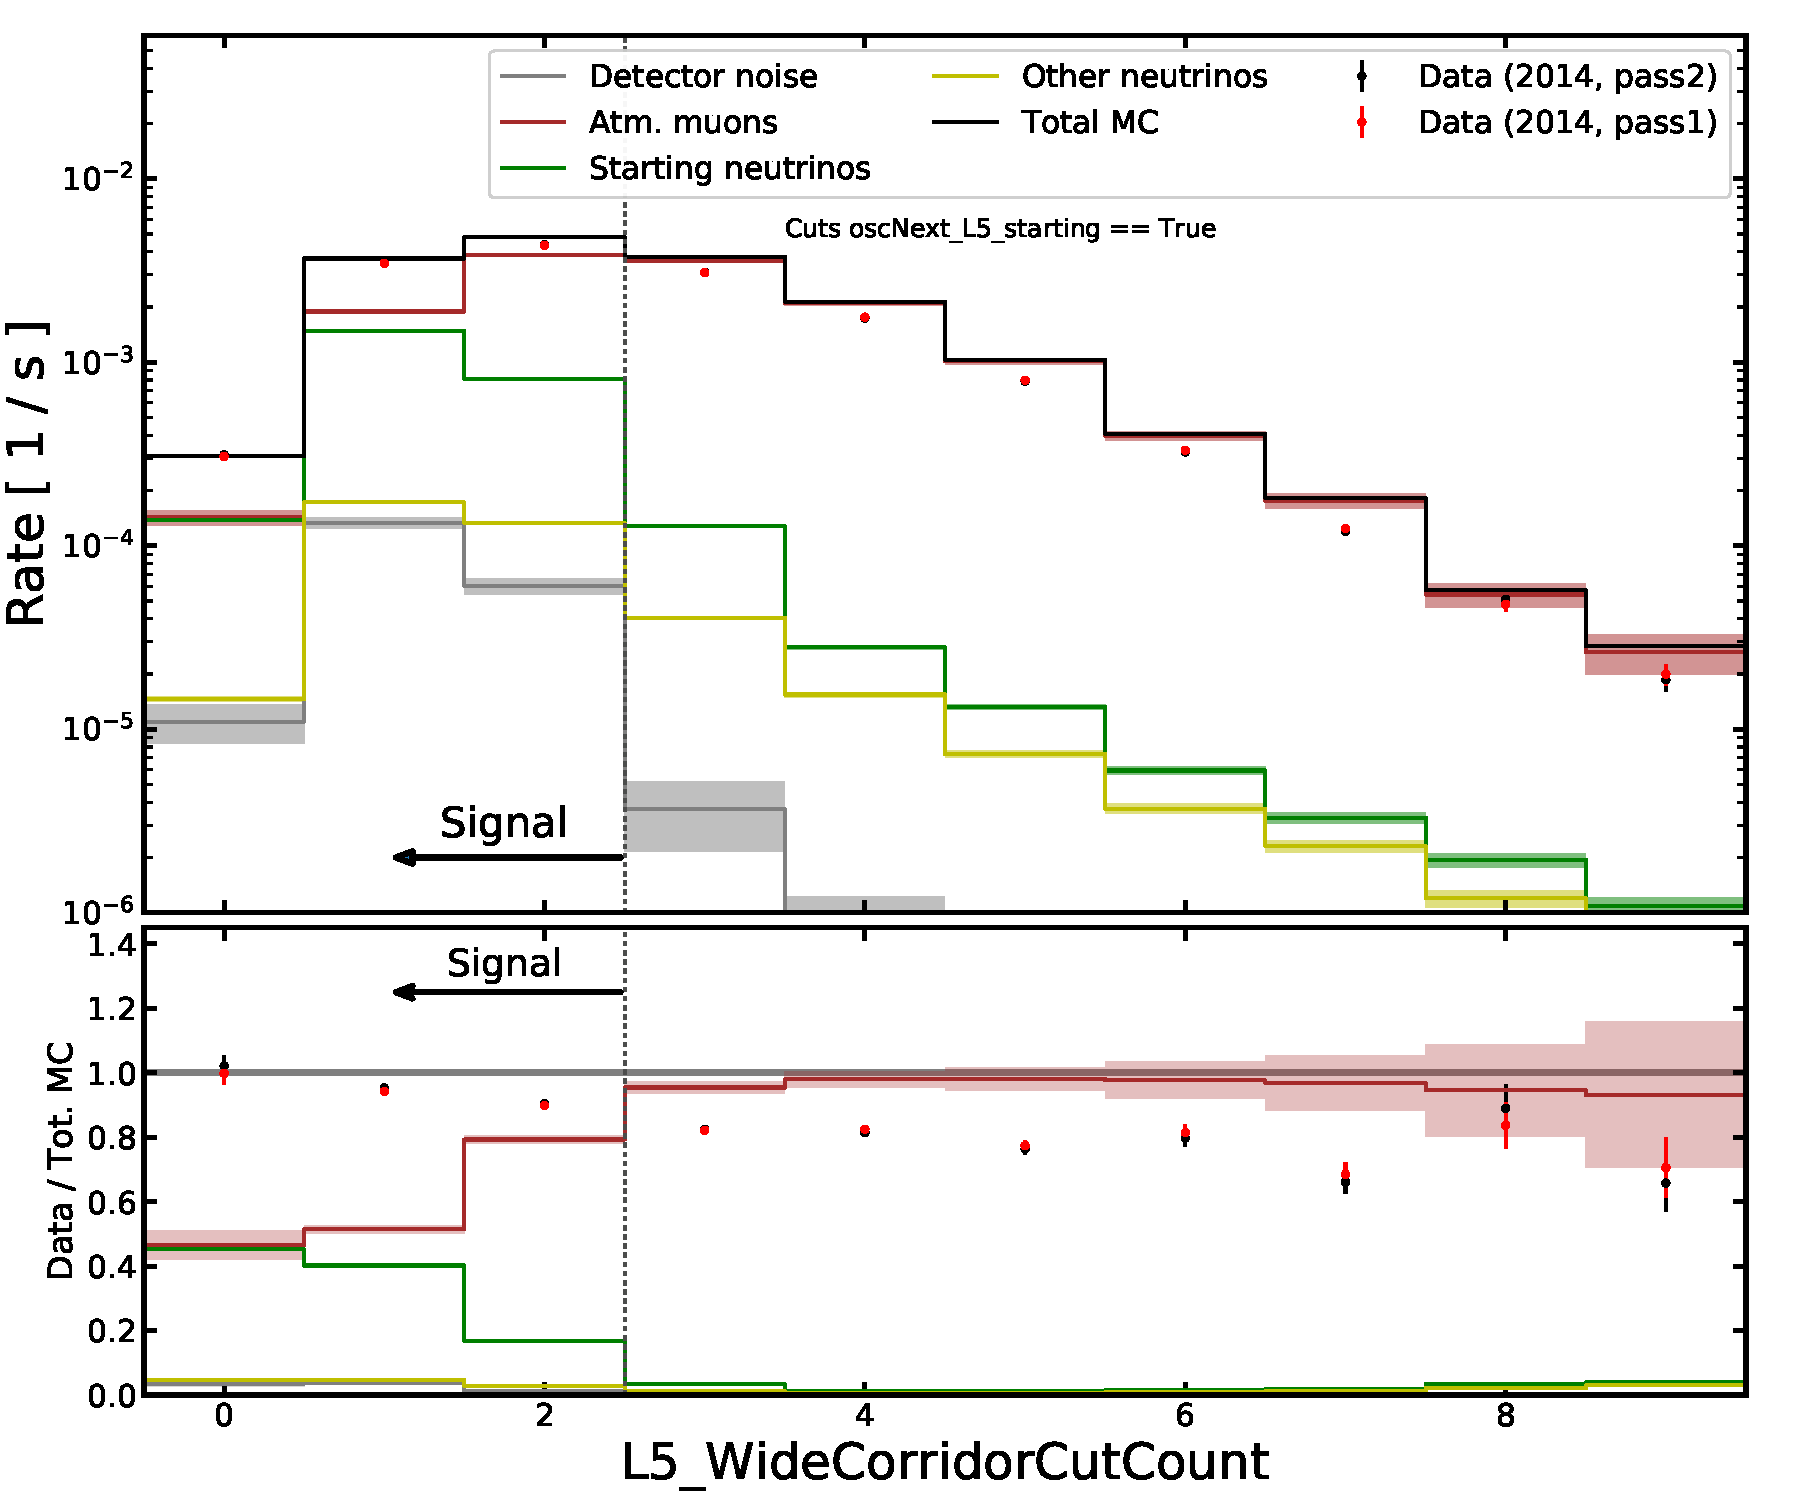
\includegraphics[width=7 cm]{figures/icecube/selection/L5_contained_L5_WideCorridorCutCount.pdf}
    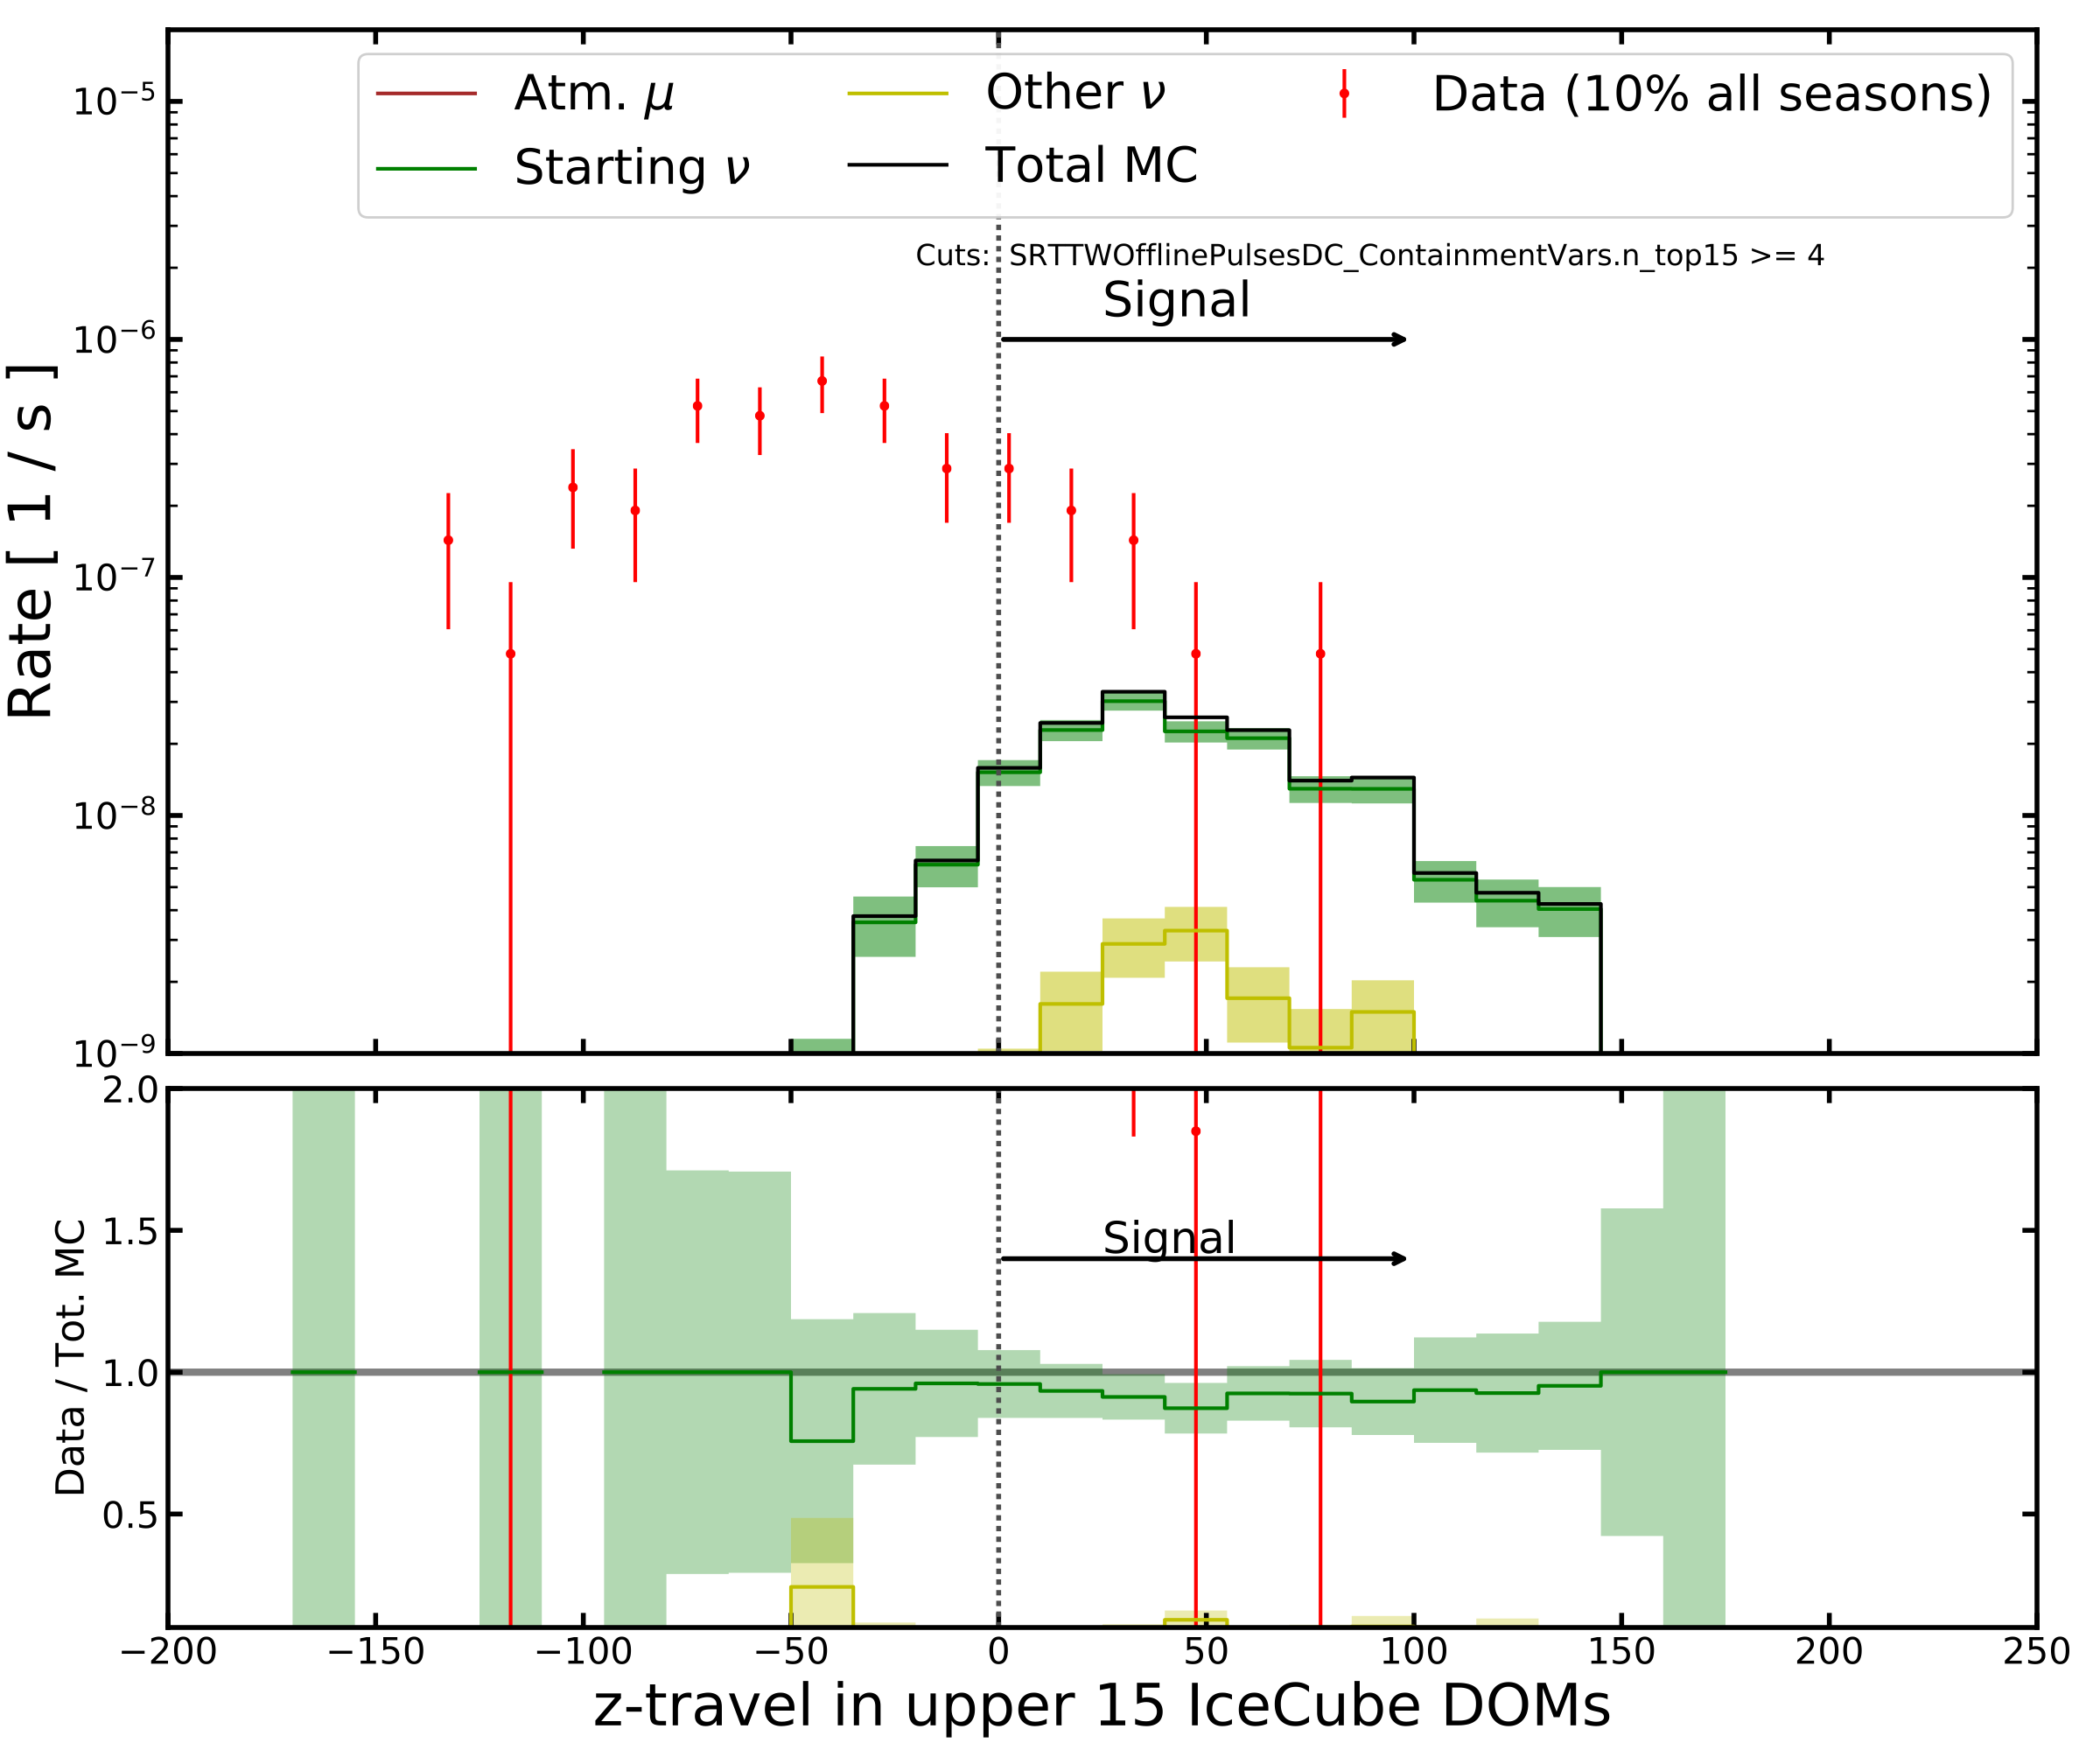
\includegraphics[width=7 cm]{figures/icecube/selection/SRTTWOfflinePulsesDC_ContainmentVars.z_travel_top15.png}
    \caption{Distributions for one of the L5 corridor cut variables (left) and one of the variables used to reject coincident muon events (right). The distribution in the right panel is shown only for events which have at least four hits in the uppermost 15 DOMs combined over all IceCube strings.}
    \label{fig:l5-vars}
\end{figure*}

\begin{table}
\begin{tabular}{lrrrrr}
Event type  & DC filter   & L3   & L4   & L5   & Eff. (\%) \\
\toprule
Atm. $\mu$         & 7273 & 505  & 28.1 & 0.93 & 0.012          \\
Pure noise         & 6621 & 36.6 & 0.28 & 0.07 & 0.001          \\
Atm. $\nu_e$ CC    & 1.61 & 0.95 & 0.84 & 0.48 & 29.8           \\
Atm. $\nu_\mu$ CC  & 6.16 & 3.77 & 3.11 & 1.39 & 22.5           \\
Atm. $\nu_\tau$ CC & 0.19 & 0.13 & 0.12 & 0.07 & 36.8           \\
Atm. $\nu$ NC      & 0.86 & 0.53 & 0.46 & 0.23 & 26.7  \\
\end{tabular}
\caption{Summary of the rates (in mHz) obtained after each level of selection. Neutrinos are weighted to an atmospheric spectrum with oscillations included.}
\label{tab:l5_summary}
\end{table}

\subsection{Event Reconstruction}
\label{sec:event-reconstruction}

After the L5 selection, the rate of muons is reduced enough such that the majority of the total sample is expected to consist of atmospheric neutrinos, and it is at this point that the event reconstruction and signature classification is run. For the measurement presented in this thesis, three reconstructed quantities are required: The zenith angle, the energy, and a proxy score that determines the flavor of a neutrino. As described in section \ref{sec:particle-signatures}, all neutrino events in DeepCore can be effectively approximated as either a cascade ($\nu_e$ CC events, all NC events, and 83\% of $\nu_\tau$ CC events) or a combination of a cascade at the neutrino interaction point with an out-going muon track ($\nu_\mu$ CC events and 17\% of $\nu_\tau$ CC events). The zenith angle can be most accurately reconstructed for track-like events due to their elongated, highly directional signature. For cascades, the reconstruction of the direction is more difficult because of their most compact and diffuse light distribution. The energy of a neutrino event is reconstructed by comparing the expected light output of a combined track and cascade hypothesis to the observed hits. Finally, the flavor proxy is calculated using variables that characterize the elongation of the observed hit signature  and the goodness-of-fit of a combined track and cascade hypothesis compared to that of a cascade-only hypothesis. The resulting score allows the separation of muon neutrino interactions from other interactions, which is ideally suitable to observe the muon neutrino disappearance oscillation channel.

\subsubsection{Zenith angle reconstruction}
The zenith angle is reconstructed using the Single-string Antares-inspired Analysis (\textsc{santa})\sidecite{Garza2014Measurement}. It is an older algorithm aimed at reconstructing the direction of muon tracks that has been originally developed for use in the ANTARES neutrino telescope~\sidecite{Aguilar:2011zz}. It has since been refurbished and improved in IceCube as described in detail in~\sidecite{lowen-reco-paper}.

The reconstructed pulse series in every DOM is summarized by the time of the first pulse and the sum of charges of all pulses. This time and charge is the only information used by the reconstruction and is referred to as a \emph{hit} in the following. The first step of the  reconstruction algorithm is a cleaning routine that removes hits produced
by photons that have been scattered many times as they traveled
through the ice, leaving only hits from photons that have travelled in approximately straight lines based on the time difference between hits on the same string.
%The algorithm is a simplification from an earlier implementation described in \cite{Garza2014Measurement}.
It calculates the signal speed between hits on the same string, and removes a hit if this velocity is below the speed of light in ice. This is a simplification from the algorithm described in \cite{Garza2014Measurement}, where the effective signal velocity was updated during the selection process. The selection is run separately for each string, and if fewer than three hits remain on a string, all hits on the string are discarded. In total, it is necessary that at least five hits remain in an event in order to run the directional reconstruction. If only hits on one string remain after the selection, the event is referred to as a \emph{single-string} event, otherwise it is a \emph{multi-string} event. The reconstruction is generally more accurate for multi-string events, because the spacing between strings provides a long lever arm to constrain the direction of a track.

The directional reconstruction itself is a modified $\chi^2$-regression with respect to the observed and predicted observation time with an additional regularization term involving the observed charge, where the expected arrival time for unscattered Cherenkov photons is calculated geometrically under the assumption of an infinitely long track without stochastic energy losses.

% \subsubsection{Hit selection}

% \label{sub:hit-selection}The first step of the \textsc{santa} reconstruction
% is the selection of minimally scattered photons from all of the observed
% pulses by removing those pulses within the trigger window that are likely to have undergone a significant amount of scattering.

% We combine the pulse series recorded by each activated DOM to a \emph{hit} with the time of the first pulse and the total charge of all pulses. All subsequent cleaning and reconstruction steps are applied to these combined hits. To remove scattered light, we make use of the fact that the largest possible delay between hits that are produced by \emph{unscattered} light on two different DOMs, $i$ and $j$, on the same string, is the time it takes for a directly up- or down-going light front to travel from one DOM to the other, $\tau_{ij}=|\Delta z_{ij}|/c_{\mathrm{ice}}$, where $|\Delta z_{ij}|$ is the distance between DOMs $i$ and $j$ and $c_{\mathrm{ice}}$ is the speed of light in ice. If the time delay between two hits, $\Delta t_{ij}$, is larger than the maximum delay, $\tau_{ij}$, then we know that the light must have undergone some amount of scattering. As a starting point for the hit selection, we choose the hit with the highest charge on each string, $i=0$, and first remove any earlier hit, $j$, where $-\Delta t_{0j} > \tau_{0j}$. From there, the algorithm iterates through every hit, $i$, and removes any other hit, $j$, where $\Delta t_{ij} > \tau_{ij}$. If fewer than 3 hits remain on a string, the entire string is removed from the event. If less than 5 hits remain in the event, it cannot be reconstructed. This is a simplified version of the cleaning procedure described in Ref.~\cite{Garza2014Measurement} and leaves more scattered light in the events. This is compensated for by the addition of the robust loss function (Sec.~\ref{sec:robust-losses}). In this configuration, we can reconstruct about 10\% more \numucc events than with the original implementation~from Ref.~\cite{Garza2014Measurement} at a similar resolution. In the example event fits in Figs.~\ref{fig:santa-single-string-example} \& \ref{fig:santa-multi-string-example}, the hits that are removed by the hit selection are crossed out.


% \subsubsection{Single-String vs. Multi-String}

% After the hit-cleaning procedure, passing events fall
% into two basic categories that are reconstructed differently. The first category is \emph{multi-string}
% events that contain observed charges in modules on two or more strings
% of the detector. Since a string is removed entirely from an event
% if it has less than three hits left after hit cleaning, a multi-string
% event contains at least six modules with recorded charges: three on
% one string and three on another string. In these events, we reconstruct both the
% zenith and the azimuth angles of the direction of a track. The second category is \emph{single-string} events that contain only one string in which modules have observed charges. Since all modules on a single string share approximately the same $x$ and $y$ coordinates, the azimuth angle of a track cannot be reconstructed. Example events for single-string and multi-string event fits are shown in Figs.~\ref{fig:santa-single-string-example} and \ref{fig:santa-multi-string-example}, respectively.

% \begin{figure}[h]
%     \centering
%     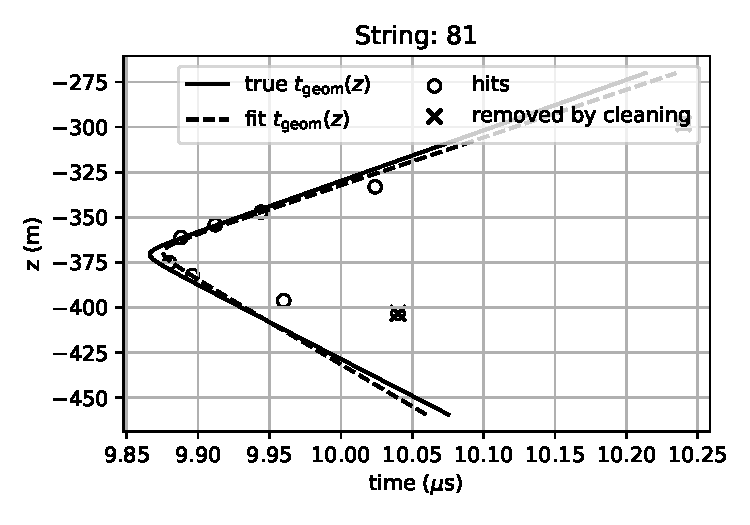
\includegraphics[width=\linewidth]{figures/santa/single_string_example_with_cleaning_id_29130693.pdf}
%     \caption{Example of a \numucc event reconstructed with \textsc{santa} on a single string. Circles show each hit, where the z-coordinate is the position of the DOM and the time is the time of the first observed pulse in that DOM.}
%     \label{fig:santa-single-string-example}
% \end{figure}

% \begin{figure*}[ht]
%     \centering
%     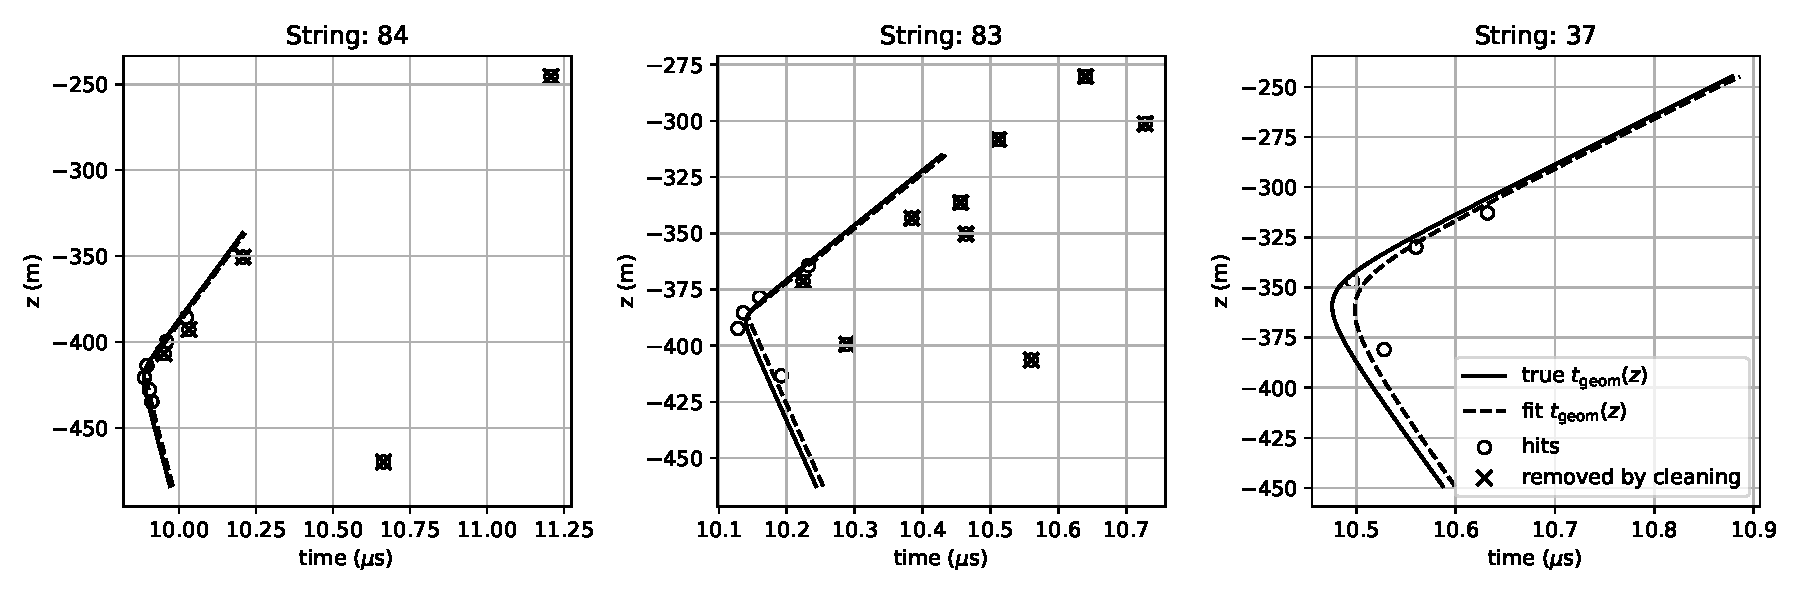
\includegraphics[width=\textwidth]{figures/santa/multi_string_example_with_cleaning_id_12607962.pdf}
%     \caption{Example of a \numucc event reconstructed with \textsc{santa} with hits on several strings. Strings 84, 83 and 37 are spaced $\sim80\,\mathrm{m}$ apart from each other and form a highly obtuse triangle.}
%     \label{fig:santa-multi-string-example}
% \end{figure*}

\subsubsection{Geometry of Tracks in IceCube}
\label{subsec:geometric-time-derivation}

To perform the $\chi^{2}$-fit on the observed hit times for a track hypothesis, we first need to derive the expected photon arrival time for an optical module at position $\vec{r}=(x,y,z)$ given the parameters of the hypothesis.

We characterize a track by a normalized direction vector $\vec{u}=(u_{x},u_{y},u_{z})$,
an anchor point $\vec{q}=(q_{x},q_{y},q_{z})$ and a time $t_{0}$
at which the particle passes through $\vec{q}$. In this simplified
hypothesis, tracks are modeled as being infinite in both directions;
there are no parameters to fix the start and end position and the
velocity is fixed to the vacuum speed of light, $c$. Since the reconstruction ignores DOMs that have not recorded any pulses, the fact that the true track length is finite only makes a negligible  difference.
Without scattering, all Cherenkov photons lie on a cone with an opening
angle $\theta_{c}$ (see Fig.~\ref{fig:Detailed-track-geometry})
whose tip is at the position of the particle at the time $\vec{p}(t)$. The opening angle satisfies $\cos(\theta_c)=1/n_{\mathrm{ph}}$, where $n_{\mathrm{ph}}$ is the phase index of refraction of the ice.

\begin{figure}[h]
\begin{centering}
\tikzsetnextfilename{track_geometry_santa}%
\begin{tikzpicture}[scale=1,>=stealth]
	\path[name path=track] (0,3) -- (9,3);
	\node[shape=star,
	      star point height=1cm,
	      star point ratio=0.5,
	      draw, fill=black,
	      label=below:$\vec{p}(t_{\mathrm{em}})$] (emission) at (1,3) {};
	\draw[->, decorate,
	decoration={snake,amplitude=.4mm,segment length=2mm,post length=1mm}]
		(emission.center)
		-- node[sloped, above] {$d_{\gamma}$} +(40:4)
		node[label=above:DOM at $\vec{r}$] (dompos) {};
	\path[name path=cone] (dompos.center) -- +(-50:4);
	\draw[name intersections={of=track and cone, by=tip}]
		(dompos.center) -- node[sloped, above] {Cherenkov light cone} (tip)
		node[label=below:$\vec{p}(t_{\mathrm{geom}})$] (muonpos) {};
	\draw[fill=black, opacity=0.5] (dompos.center) circle (5pt);
	\draw[color=black, ->, style=very thick] (0,3) node[anchor=north]{muon} -- (muonpos.center);
	\draw (emission.center) +(1,0) node[anchor=south east]{$\theta_c$}  arc (0:40:1);
	\path (emission.center)
		-- node[shape=circle,
			fill=black,
			label=below:$\vec{q}$] (vertex) {}
		(tip);
	\draw[->] (vertex.center) -- node[sloped, below] {$\vec{r}-\vec{q}$} (dompos.center);
	%\draw (vertex.center) +(-1,0) arc (180:140:1);
	%\path (vertex.center) -- +(160:0.6) node {$\theta$};
	\draw[->] (vertex.center) ++(0.2, 0.2) -- node[above] {$\vec{u}$} +(1,0);
\end{tikzpicture}\par
\end{centering}
\caption{\label{fig:Detailed-track-geometry}Detailed geometry of a light cone
created by a track. $\vec{q}$ is the position of the anchor point
and $\vec{r}$ is the position of the optical module. $\vec{p}(t_{\mathrm{em}})$
and $\vec{p}(t_{\mathrm{geom}})$ are the positions of the muon at
the time the photon is emitted and when it is geometrically expected
to arrive, respectively.}
\end{figure}

% We solve the geometric equations analogously to~Ref.~\cite{Garza2014Measurement} assuming that a photon emitted by the moving particle travels in a straight line at a velocity of $c$ divided by the group index of refraction $n_{\mathrm{gr}}$, which gives the \emph{geometric time}, $t_{\mathrm{geom}}$, as a function of the track parameters

% \begin{equation}
% t_{\mathrm{geom}}=t_{0}+\frac{1}{c}\left(\left(\vec{r}-\vec{q}\right)\cdot\vec{u}+\frac{d_{\gamma}}{n_{\mathrm{ph}}}\left(n_{\mathrm{ph}}n_{\mathrm{gr}}-1\right)\right)\label{eq:t_geom-MS-track}
% \end{equation}
% where the distance traveled by the photon $d_\gamma$ is
% \begin{equation}
% d_{\gamma}=n_{\mathrm{ph}}\sqrt{\frac{1}{n_{\mathrm{ph}}^{2}-1}\left(\vec{u}\times\left(\vec{r}-\vec{q}\right)\right)^{2}}\,.\label{eq:photon-distance-3d}
% \end{equation}

% The group and phase indices of refraction depend on the wavelength, but for this reconstruction we use as value for the wavelength $\lambda=400\;\mathrm{nm}$
% \footnote{$400\;\mathrm{nm}$ is near the wavelength of the highest acceptance of the optical modules.\cite{Aartsen:2016nxy}},
% , where $n_{\mathrm{gr}}=1.356$ and $n_{\mathrm{ph}}=1.319$~from Ref.~\cite{PRICE200197}.

% \subsubsection{Fitting Procedure}
% \label{sec:santa-loss}

% For a given set of parameters $\vec{\theta}=(\vec{u},\vec{q},t_0)$, we minimize a modified chi-square loss function given by
% \begin{equation}
% L(\vec{\theta})=\sum_{i=1}^{N}r^2_i
% +
% \frac{1}{\bar{q}}\sum_{i=1}^{N}\tilde{q}_i \frac{d_{\gamma,i}}{d_0}\,.\label{eq:chi-square-mod-loss}
% \end{equation}
% where $\bar{q}$ is the average of $\tilde{q}_i$, and $r^2_i$ is the chi-square residual for each observed hit, $i$, between the observed time, $t_{\mathrm{obs}, i}$ and the geometric arrival time, $t_{\mathrm{geom},i}(\vec{\theta})$,

% \begin{equation}
% r_{i}^{2}=\left(\frac{t_{\mathrm{geom},i}(\vec{\theta})-t_{\mathrm{obs},i}}{\sigma_{t}}\right)^{2}\,.
% \end{equation}

% The uncertainty on the pulse time measurement is approximately $\sigma_{t}=3\,\mathrm{ns}$, corresponding to the readout rate of the modules~\cite{Abbasi:2008aa}.

% The second term in eq.~\ref{eq:chi-square-mod-loss} is a regularization term that multiplies the distance traveled by a photon to the optical module that recorded it, $d_{\gamma,i}$, by the measured charge, $\tilde{q}_i$, to penalize solutions where a large charge is observed far away from the hypothesized track position. Because the modules are most sensitive on the side facing towards the bedrock, we correct the observed total charge in each DOM, $q_i$, for the sensitivity with
% \begin{equation}
% \tilde{q}_i=q_i\frac{2}{1+\cos(\vartheta_i)}\,,
% \end{equation}
% where $\vartheta_i$ is the angle between the direction of the photon
% and a vector pointing up to the surface of the ice.
% The parameter $d_{0}$ determines the relative contribution of the regularization term. Its value has been optimized for best average performance of the reconstruction and is fixed to $7\,\mathrm{m}$. 

% \subsubsection{Robust loss functions }
% \label{sec:robust-losses}
% After the hit selection described in Sec.~\ref{subsec:hit-selection}, a small number of hits from photons that have undergone significant amounts of scattering will remain that could strongly bias the fit result. We improve the robustness of the regression against such outliers by wrapping the squared residuals for each pulse in eq. \ref{eq:chi-square-mod-loss}, $r^{2}_i$, 
% with the Cauchy robust loss function
% \begin{equation}
% r_i^2 \rightarrow \phi(r_{i}^{2})=\log\left(1+r_{i}^{2}\right)\,.
% \label{eq:cauchy-loss}
% \end{equation}
% It reproduces the original $r^{2}$ residual
% for small values of $r$, but grows more slowly than $r^2$ for large values of $r$, so that outliers are effectively given less weight.

% Additionally, we choose the point of a “soft cut-off”,
% denoted herein as $C$, at which the residual diverges from the regular $r_{i}^{2}$
% in units of standard deviations by setting 
% \begin{equation}
% \phi(r_{i}^{2})\rightarrow\phi\left(\nicefrac{r_{i}^{2}}{C^{2}}\right)C^{2}\,.
% \end{equation}

% Figure~\ref{fig:robust-losses-example} shows the Cauchy loss function
% for different values of $C$.  The choice of the value of $C$ is a trade-off. If it is too large, then the fit can be strongly influenced by single outliers. If it is too small, then the fit ignores too many hits and falls into degenerate solutions. We found the optimal value to be $C=3$. At this setting, the fit can effectively ignore hits that are far away from the Cherenkov cone.

% % \begin{figure}[h]
% % % \begin{centering}
% % \centering
% % \includegraphics[width=8cm]{figures/santa/cauchy_loss_c.pdf}
% % % \par\end{centering}
% % \caption{\label{fig:robust-losses-example}The Cauchy robust loss function for different values of the scaling parameter, $C$. In a $\chi^{2}$
% % fit, the residual is the difference between the model and the observation
% % in units of standard deviations, $r=\frac{x-\mu}{\sigma}$ .}
% % \end{figure}
% As a further constraint on the regression, we apply the robust loss function from eq.~\ref{eq:cauchy-loss} only to pulses where the observed time is later than the expected photon time, since we expect that scattering would only cause photons to arrive too late, never too early. 

% \subsubsection{Resolution}

% The performance of the \textsc{santa} algorithm will be presented, together with the next algorithm discussed, in Sec.~\ref{sec:performance}.

